\documentclass{bioinfo}
\copyrightyear{2019} \pubyear{2019}

\access{Advance Access Publication Date: Day Month Year}
\appnotes{Manuscript Category}

\usepackage[ruled,vlined]{algorithm2e}
\usepackage{xcolor}

\begin{document}
\firstpage{1}

\subtitle{Subject Section}

\title[BiORSEO]{BiORSEO: A bi-objective method to predict RNA secondary structures with pseudoknots using RNA 3D modules}
\author[Becquey \textit{et~al}.]{Louis Becquey\,$^{\text{\sfb 1,}*}$, Eric Angel\,$^{\text{\sfb 1}}$ and Fariza Tahi\,$^{\text{\sfb 1}*}$}
\address{$^{\text{\sf 1}}$IBISC, Univ Evry, Universite Paris-Saclay, 91025, Evry, France}

\corresp{$^\ast$To whom correspondence should be addressed.}

\history{Received on XXXXX; revised on XXXXX; accepted on XXXXX}

\editor{Associate Editor: XXXXXXX}

\abstract{\textbf{Motivation:} RNA loops have been modelled and clustered from solved 3D structures into ordered collections of recurrent non-canonical interactions called "RNA modules", available in databases. This work explores what information from such modules can be used to improve secondary structure prediction. 
We propose a bi-objective method for predicting RNA secondary structures by minimizing both an energy-based and a knowledge-based potential. The tool, called \textsc{BiORSEO}, outputs secondary structures corresponding to the optimal solutions from the Pareto set.\\
\textbf{Results:}  We compare several approaches to predict secondary structures using inserted RNA modules information: two module data sources, Rna3Dmotif and The RNA 3D Motif Atlas, and different ways to score the module insertions: module size, module complexity, or module probability according to models like JAR3D and BayesPairing. We benchmark them against a large set of known secondary structures, \textcolor{red}{including some state-of-the-art tools, and comment on the usefulness of the half physics-based, half data-based approach}.\\ % Some of the tested methods present a good performance, especially on structures containing pseudoknots. They are compared to state of the art tools for secondary structure prediction.\\
\textbf{Availability:} The software \textcolor{red}{is} available for download on the \href{https://evryrna.ibisc.univ-evry.fr/evryrna/BiORSEO/}{EvryRNA website}, as well as the datasets.\\
\textbf{Contact:} \href{louis.becquey@univ-evry.fr}{louis.becquey@univ-evry.fr}, \href{fariza.tahi@univ-evry.fr}{fariza.tahi@univ-evry.fr}\\
\textbf{Supplementary information:} Supplementary sections are available at \textit{Bioinformatics}
online.}

\maketitle

%%%%%%%%%%%%%%%%%%%%%%%%%%%%%%%%%%%%%%%%%%%%%%%%%%%%%%%%%%%%%%%%%%%%%%%%%%%%%%%%%%%%%%%%%%%%%%%%
\section{Introduction}
Ribonucleic acid (RNA) is a macromolecule which is often single-stranded. Therefore, the strand has the ability to fold in space in more complex ways than DNA, that we mostly know to form double-stranded stems. A stem is a succession of basepairs called Watson-Crick basepairs, or "canonical", stacked on top of each other. As this can still happen with RNA, we also observe several other ways for a nucleotide to interact with another. For example, Leontis and Westhof proposed a classification of 12 non-canonical basepairs~(\citealp{leontis2001geometric}). Some of the nucleotides can also interact with the 2'OH of a ribose, or with a phosphate, or even not interact at all and bulge out the RNA structure.
   
\paragraph{Modelling RNA structures as graphs} ~ 
For modelling purposes, researchers working on computational problems involving RNA represent them with graphs.  A recent article~(\citealp{schlick2018adventures}) details the different graph models of RNAs and their respective advantages. 
We are particularly interested in the secondary structure graph of the RNA, i.e. a graph where the nucleotides are nodes, and backbone bonds and canonical basepairs are edges. In this kind of graph, the non-canonical interactions do not appear. 
As the problem of predicting the 3D structure of an RNA from sequence has been too computationally expensive for years, and is still difficult, a common first step has been to predict this secondary structure (2D) graph, by computing what regions will form stems and what regions will \textcolor{red}{not be Watson-Crick basepaired}, forming so-called loops. 
In many cases, the solution to the 2D folding problem is not unique, and RNAs have the ability to switch between several metastable conformations. Most approaches use dynamic programming schemes to compute the RNA partition function and/or canonical pairing probabilities, i.e. the probability for each nucleotide to form a canonical base-pair with every other nucleotide, or to remain unpaired~(\citealp{mccaskill1990equilibrium}). Once the  partition function is computed, several models exist to rebuild one or several best structure(s): we can choose the Minimum Free Energy (MFE) structure, the one that maximizes expected accuracy (MEA), or the centroid of the ensemble. The most used implementations are some low complexity implementations such as \texttt{RNAFold} and \texttt{Fold}~(\citealp{lorenz2011viennarna}, \citealp{mathews2004using}). An important limitation of these algorithms is their inability to model so-called \textit{pseudoknotted} structures, i.e. structures with basepairs $(i,j)$ and $(k,l)$ when $i<k<j<l$. 
Later, some variants taking pseudoknots into account were developped, e.g. in the NUPACK package~(\citealp{dirksAlgorithmComputingNucleic2004}) or \texttt{ProbKnot} from the RNAstructure package~(\citealp{bellaousov2010probknot}).
We can also cite Biokop (\citealp{legendre_bi-objective_2018}), a recent tool that uses both MFE and MEA criterions in a bi-objective framework, and returns optimal and suboptimal structures including pseudoknots.

RNAs can be seen as an assembly of stems and loops. To move from the planar 2D graph to 3D, one usually predicts the 3D structure of stems and loops separately. Stems are relatively easy to tackle because of the isostericity of the Watson-Crick basepairs; their structure has been widely observed and features low variability. On the other hand, to accurately model loops in 3D, one needs to take the non-canonical interactions into account. In many cases, two hairpin loops can even form new canonical basepairs to form \textit{kissing hairpins}, a particular pseudoknot type (called HHH) which is hard to predict because it involves a distant basepair between two unpaired loop regions. More nomenclature details about loops and pseudoknots are provided in Supplementary Section~A.

\paragraph{\textcolor{red}{Modelling loops as modules}} ~  Several works have gathered 3D crystal structures involving RNA chains, extracted the loops from those RNA chains and annotated the base contacts using MC-Annotate (\citealp{gendron2001quantitative}), FR3D (\citealp{sarver_fr3d:_2008}) or DSSR (\citealp{lu_dssr:_2015}). 
They model the loops with more detailed graphs describing non-canonical contacts on their edges. 
The graphs can then be clustered with respect to a similarity or isomorphism measure, and the sequence variations over the nucleotides of the loop can be modeled. 
Those models are called RNA \textit{modules}, i.e. an ordered collection of non-canonical basepairs or stacking interactions, leading to a conserved 3D shape in different RNA molecules. 
We can cite the work from (\citealp{djelloul_automated_2008}) with Rna3Dmotif, a pipeline that extracts terminal hairpin loops (HL), internal loops (IL), and multiple loops (ML) from structures annotated by FR3D, and can cluster them using a graph similarity metric. 
Another one is the RNA 3D Motif Atlas~(\citealp{petrov_automated_2013}), which does not support multiple loops, but clusters the loops using all sequence information, nucleotide contacts and shape information, which leads to loop module models with tolerance in sequence and length variations. 
\textcolor{red}{More recent ones are RNAMotifClusters (\citealp{ge2018novo}), and also} CaRNAval (\citealp{reinharz2018mining}), an approach that enables to model a wide variety of structural features such as multipairs, multi-stranded loops, and pseudoknots. 
To be exhaustive, we also can cite RNA Bricks 2 (\citealp{chojnowski2014rna}), which has the particularity to also study contacts with protein chains. 

\textcolor{red}{Further work has been done to help researchers detecting if some RNA sequence folds following some known module model, user-provided, or searched in a database.}
For example, JAR3D (\citealp{zirbel_identifying_2015}) can score the modules from the RNA 3D Motif Atlas against a query \textcolor{red}{loop} sequence. 
\textcolor{red}{With RMDetect~(\citealp{cruz2011sequence}), the authors proposed to build bayesian networks from any RNA module's graph to summarize all the observed sequence variants of the module. 
The metaRNAmodules pipeline (\citealp{theis2013automated}) can then be used to build bayesian networks for Djelloul \& Denise's modules and detect them in aligned RNA sequences.  
The recent BayesPairing tool (\citealp{sarrazin2019automated}) can do the same for modules from several databases, and allows to detect them in single RNA sequences.}

\paragraph{\textcolor{red}{Secondary structure prediction using RNA modules}} ~ In this paper, \textcolor{red}{we want to test if the knowledge that a subsequence matches well some module model helps identifying a loop in the RNA, when predicting the secondary structure.} 
In other words, we do not use the 3D data to \textcolor{red}{propose 3D conformations for the loops}, but we use it to score 2D conformations. 
A first attempt \textcolor{red}{to use modules to guide RNA 2D structure predictions} is RNA-MoIP~(\citealp{reinharz_towards_2012}). 
The tool \textcolor{red}{inserts modules from Rna3Dmotif in a set of candidate solutions} (often given by a simple tool like RNAsubopt~(\citealp{lorenz2011viennarna})) to \textcolor{red}{return a single} 2D structure with non-canonical base-pairs included, \textcolor{red}{which is then a better input} to give to the 3D reconstruction tool MC-Sym~(\citealp{parisien2008mc}), resulting in better prediction of 3D structures. 
\textcolor{red}{Another example is the use of JAR3D and metaRNAmodules by (\citealp{theis2015rna}) to predict secondary structures at genome-wide scale, using an alignment of 13 genomes. 
This last study shows the use of modules lowers the false discovery rate of secondary structure elements. 
This is encouraging, but as we focus more on short, unaligned single RNA sequences, we compare ourselves to RNA-MoIP in this study. 
Going further than metaRNAmodules, BayesPairing allows to detect modules from more databases and without sequence alignments, so we are rather considering it in this work.}

\textcolor{red}{When inserting modules into secondary structures, RNA-MoIP sometimes has to break basepairs. 
It tries to find a compromise between staying close to the initial structure, and insert more modules. Unfortunately, }it cannot distinguish important base-pairs from less important ones, and might break some of the ones stabilizing a whole stem while inserting a module, resulting in less probable structures as output. \textcolor{red}{Evidence is provided in Supplementary Section B.}
To \textcolor{red}{overcome this problem}, we design a method which builds a 2D structure by simultaneously placing base-pairs and modules in a single step, taking into account two objectives: the expected accuracy of the structure in the equilibrium ensemble fold, and a custom function that reflects the number and quality of inserted modules (several models are studied). 
This method leads to our new tool BiORSEO (Bi-Objective RNA Structure Efficient Optimizer). 
Our approach avoids using a weighted linear combination of the objectives as done in RNA-MoIP (which can miss interesting \textcolor{red}{so-called \textit{non-supported} solutions}). In this paper, we use a bi-objective Pareto-based approach, i.e. we identify all the non-dominated structures (the structures for which no other structure scores better on the two objectives).\\

The paper is organized as follows. In the next section, we present the module models sources, the insertion models and some objective functions, and the procedure to compare them. Then we present a benchmark of all those variants against reference tools in Section \ref{sec:results}, using two reference datasets. \textcolor{red}{We also discuss on the usefulness of the module criteria.}

\begin{figure*}[t]
   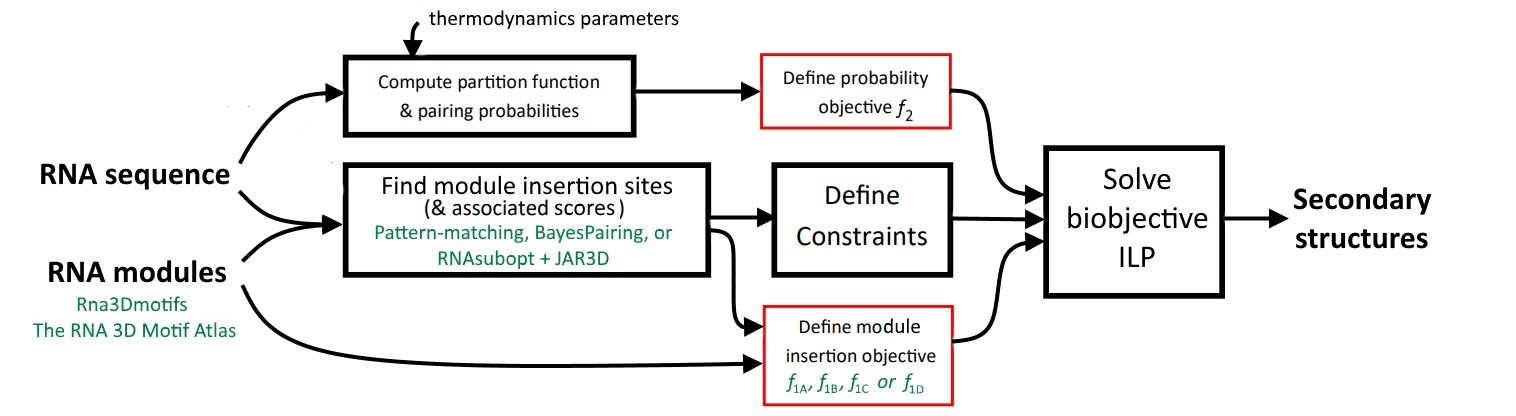
\includegraphics[width=\textwidth]{graph_abstract.jpg} 
   \caption{The information flow in our method. The inputs are the RNA sequence and module models from a database. First, we compute the pairing probabilities based on~(\citealp{dirksAlgorithmComputingNucleic2004}) and the probable insertion sites using 3 different methods listed in Section \ref{sec:models}. Then, we can define two objectives and linear constraints to compute the Pareto set of secondary structures for the input sequence, by solving a bi-objective integer linear program (ILP).}
   \label{fig:pipeline}
\end{figure*}

%%%%%%%%%%%%%%%%%%%%%%%%%%%%%%%%%%%%%%%%%%%%%%%%%%%%%%%%%%%%%%%%%%%%%%%%%%%%%%%%%%%%%%%%%%%%%%%%
\begin{methods}
\section{Methods}\label{sec:methods}
We compare two databases of modules: (1) the module data-set used by RNA-MoIP ~(\citealp{reinharz_towards_2012}), in the DESC file format of Rna3Dmotif~(\citealp{djelloul_automated_2008}); (2) modules from the RNA 3D Motif Atlas v3.2, as provided on the BGSU website, see~(\citealp{petrov_automated_2013}) for more information. Our main procedure is the following:
\begin{itemize}
\item \textbf{Pattern-matching step:} Find all possible occurrences of known RNA modules in the query sequence, by finding subsequences of the query that score well with the probabilistic models of the modules (several models are compared).
\item \textbf{Constraints definition step:} Define constraints on the secondary structure imposed by modules if they would be included (in this case, \textcolor{red}{the closing basepairs of the module are mandatory}).
 \item \textbf{Optimization step:} Find a secondary structure that satisfies as much as possible both the expected accuracy of the structure and a criterion taking into account module inclusions, by solving a bi-objective integer linear programming (ILP) problem, using the constraints defined in the previous step.
\end{itemize}
 
The ILP framework used to define the constraints and solve the resulting optimization problem is similar to previous works like IPknot (\citealp{sato_ipknot:_2011}), RNA-MoIP~(\citealp{reinharz_towards_2012}) or Biokop (\citealp{legendre_bi-objective_2018}).
We chose the ILP approach because it has proven its outperformance with IPknot and Biokop when it comes to pseudoknot prediction, see (\citealp{legendre_bi-objective_2018}). In particular, any type of pseudoknot can be predicted. 

Figure \ref{fig:pipeline} summarizes the \textcolor{red}{whole} procedure on a graphical pipeline.

\subsection{Pattern matching step}\label{sec:models}
Several methods have been proposed to determine if a sequence (or a part of it) is likely to fold following a given module. \textcolor{red}{We benchmarked the following ones:}

\paragraph{Direct pattern matching} ~ The simplest approach when no statistical model is available is to use a regular expression and direct pattern matching against the input sequence. This is the approach used by RNA-MoIP. We used it with the Rna3Dmotif data as presented in RNA-MoIP's article ~(\citealp{reinharz_towards_2012}), dealing with special cases in the same way (very short components, wildcards).

\paragraph{JAR3D} ~ For each motif group in the RNA 3D Motif Atlas, \textcolor{red}{~(\citealp{zirbel_identifying_2015}) built} a probabilistic model for sequence variability. 
Their implementation, called JAR3D, takes user-provided loop sub-sequences in input and outputs a score for every motif of the Atlas on every provided loop. This method has the advantage to allow variations in sequence length compared to the module model. Unfortunately, it can only be used for hairpin and internal loops. Another major drawback is that it requires the computation of the pairing probabilities to first locate \textit{where} the most probable loops are, to give them as input to JAR3D. We therefore use RNAsubopt first to get the positions of the probable loops. JAR3D has been developed for modules from the RNA 3D Motif Atlas and can only be tested with them.

\paragraph{\textcolor{red}{BayesPairing's sequence probability distributions}} ~ When we have data for several instances of a module, we can estimate a probabilistic distribution of the nucleotides over the module nodes. A first intuitive approach is to use the base frequencies. But as paired nucleotides are not independent at all, it is more rigorous to model those dependencies. An approach proposed in ~(\citealp{cruz2011sequence}) is to transform the module's graph into a Bayesian network, which models the dependencies between nucleotide probabilities at every node of the graph. 
\textcolor{red}{BayesPairing~(\citealp{sarrazin2019automated}) automates the building of bayesian networks for every module.}
A large number of sequences are sampled using the Bayesian network, and they are pattern-matched against the query to find occurrences. 
An additional step compares the free energy of the structure with and without the constraint of each matched module, and selects only the candidate sites that do not deteriorate too much the energy. 
This last step is \textcolor{red}{not required here}, first because it \textcolor{red}{repeats the calculation} of the partition function, and then because we would try to insert modules \textcolor{red}{with BiORSEO} that were pre-selected \textcolor{red}{by BayesPairing} to be appropriate. 
Therefore we chose to ignore this last step and let our optimizer select the pertinent modules in the candidates. BayesPairing can be used for both data sources.


%%%%%%%%%%%%%%%%%%%%%%%%%%%%%%%%%%%%%%%%%%%%%%%%%%%%%%%%%%%%%%%%%%%%%%%%%%%%%%%%%%%%%%%%%%%%%%%%%%%%
\subsection{Constraints definition step and IP model} \label{sec:ip}
The full list of variables we used to model the problem in an integer linear program and the linear formulation of each constraint are detailed in Supplementary Section C. Here we propose different objective functions to score the candidate module insertions. %, whose performances are compared in section \ref{sec:results}.

\paragraph{Notations} ~ We call \textit{component} a piece of strand which forms an unpaired portion of a module. A HL has one, an IL or bulge has two, and a ML has more (see Supplementary Section A). Components of a module are linked together by canonical base-pairs at their extremities to form a loop. Let $x$ be a module which could be inserted at some defined position in the sequence. Let $\|x\|$ be the number of components of this module, and $k_{x,i}$ the nucleotide count of the $i$th component of $x$. When a scoring model is used (JAR3D or BayesPairing), we denote $p(x)$ the score value of $x$ inserted at the defined position. Let $p_{uv}$ be the probability for nucleotides $u$ and $v$ (with $v>u+3$) to form a canonical base-pair. We use NUPACK's dynamic programming scheme~(\citealp{dirksAlgorithmComputingNucleic2004}), which supports pseudoknots, to compute such probabilities. We denote $y^u_v$ the binary decision variable indicating that these nucleotides do form a canonical base pair, and $C^x_1$ the decision binary variable indicating whether the module $x$ will be inserted or not. The resolution of the ILP outputs solutions by fixing definitive values for the different $y^u_v$ and $C^x_1$. 

\paragraph{Objective functions} ~ The more modules that are included, the more information about set and unset base-pairs, and eventually about tertiary folds of the loops in space. 
So maximizing the number of modules could be a valid criteria. But, a disadvantage of such a criteria is that it penalizes MLs with large $\|x\|$, because the insertion of a ML forbids at the same time the insertion of several ILs or bulges in place. 
RNA-MoIP uses the sum of the squared nucleotide count over the components to try to encourage large modules~(\citealp{reinharz_towards_2012}). This is our first benchmarked criteria $f_{1A}$. 
Conversely, we could also try to maximize the number of components $\|x\|$ in the module. 
Then, we \textcolor{red}{also could} penalize a module insertion by the logarithm of the number of nucleotides involved in the looped zone (sum of the $k_{x,i}$) to avoid very long unpaired zones. 
We introduce such a penalty in criteria $f_{1B}$. We also define two more criteria, $f_{1C}$ which uses only the score returned by JAR3D or BayesPairing, and $f_{1D}$ which includes all the presented terms. 
Let $X$ be the set of all our decision variables, then the different objective functions to maximize are:
\begin{equation}f_{1A}(X) = \sum_{x} \sum_{i=1}^{\|x\|} k_{x,i}^2 \times C^x_1\label{eq:A}\end{equation}
\begin{equation}f_{1B}(X) = \sum_{x} \left[ \frac{\|x\|}{\log_2(\sum_{i=1}^{\|x\|}k_{x,i})} \times C^x_1 \right] \label{eq:B}\end{equation}
\begin{equation}f_{1C}(X) = \sum_{x} p(x) \times C^x_1 \label{eq:C}\end{equation}
\begin{equation}f_{1D}(X) = \sum_{x} \left[ \frac{\|x\|}{\log_2(\sum_{i=1}^{\|x\|}k_{x,i})} \times p(x) \times C^x_1 \right]\label{eq:D}\end{equation} \\
Regarding the second objective, aimed at maximizing the expected accuracy of the structures, we use $f_2(X) = \sum y^u_v \times p_{uv} \times I[p_{uv}>\theta]$. As first proposed by~(\citealp{sato_ipknot:_2011}), $f_2$ uses a parameter $\theta = 0.001$ to ignore very unlikely base-pairs. This prevents the explosion of the number of variables and allows a fast resolution of the IP problem.

%%%%%%%%%%%%%%%%%%%%%%%%%%%%%%%%%%%%%%%%%%%%%%%%%%%%%%%%%%%%%%%%%%%%%%%%%%%%%%%%%%%%%%%%%%%%%%%%%%%%
\subsection{Optimization step}
We use a simple dichotomic search algorithm (presented in Figure \ref{fig:findP}) to find the Pareto set of the bi-objective problem. On the first pass of the dichotomy, it solves iteratively a mono-objective problem with a constraint on the second objective, requiring it to be in an interval $[\lambda_{min}, \lambda_{max}]$. For example, if we decide to maximize objective 1; every-time a new non-dominated solution is found, $\lambda_{min}$ is set just above the new solution's objective 2 value. We then search and find another solution with a worse objective 1 value but a higher objective 2 value than previously found solutions. The second pass of the dichotomy searches below newly found solutions. In fact, it is required to search for superposed solutions to Pareto optimal ones. This is important when the criteria used to rank inserted modules is not able to separate them very well; many solutions therefore get the same $f_1$ score. This algorithm is implemented  in C++ using the CPLEX solver concert technology (\href{https://www.ibm.com/analytics/optimization-modeling-interfaces}{ILOG CPLEX Optimizer 12.8}).
\begin{figure}[!tbp]
\begin{algorithm}[H]
F:= $\emptyset$\;
\tcp{find the extrema of the Pareto front:}
L1:= maximize($f_1$, $-\infty$, $+\infty$, F)\;
L2:= maximize($f_2$, $-\infty$, $+\infty$, F)\;
\tcp{Add L1 to the results:}
\textit{R} := $\{$L1$\}$\;
\tcp{search on top of L1:}
search\_between($f_2(\text{L1}) + \epsilon$, $f_2(\text{L2})$)\;
\tcp{search if solutions superposed to L1 exist:}
search\_between($-\infty$, $f_2(\text{L1})$)\;
\Return{R}\;
\caption{FindParetoSet()}
\end{algorithm}

\begin{algorithm}[H]
$s$:= maximize($f_1$, $\lambda_{min}$, $\lambda_{max}$, F)\;
\If{$s \neq \emptyset$}{
   F:= F $\cup \{s\}$\;
   \If{$\nexists x \in R$ \textcolor{red}{such that} $x>s$}{
         \tcp{solution is undominated, add it to \textit{R}}
       \textit{R} := \textit{R} $\cup \{s\}$\;
       \While{$\exists x \in R$ \textcolor{red}{such that} $s>x$}{
             \tcp{remove dominated solutions}
           \textit{R} := \textit{R}$\setminus \{x\}$\; 
       }
         \tcp{search on top of $s$}
       search\_between($f_2(s) + \epsilon$, $\lambda_{max}$)\;
       \If{$\lambda_{max} - \lambda_{min} > \epsilon$}{
             \tcp{search if another solution superposed to $s$ exists}
           search\_between($\lambda_{min}$, $f_2(s)$)\;
       }
   }
}
\caption{search\_between($\lambda_{min}$, $\lambda_{max}$)}
\end{algorithm}

\caption{The dichotomic search algorithm to find the Pareto set. F is the ensemble of already-found structures which grows over time, and that we forbid the solver to find again. R is the set of Pareto-optimal solutions. L1 and L2 are the best solutions to the mono-objective problems regarding $f1$ and $f2$. $\mathbf{maximize}$($f$, $\lambda_{min}$, $\lambda_{max}$, F) is a procedure that \textcolor{red}{maximizes} the function $f$ (mono-objective IP problem) under the constraint that the other one has to be in interval $[\lambda_{min}$, $\lambda_{max}]$, and with the solutions in F forbidden. The inequality sign $a>b$ between two solutions denotes that solution $a$ dominates solution $b$.}\label{fig:findP}
\end{figure}
\end{methods}

%%%%%%%%%%%%%%%%%%%%%%%%%%%%%%%%%%%%%%%%%%%%%%%%%%%%%%%%%%%%%%%%%%%%%%%%%%%%%%%%%%%%%%%%%%%%%%%%%%%%
%%%%%%%%%%%%%%%%%%%%%%%%%%%%%%%%%%%%%%%%%%%%%%%%%%%%%%%%%%%%%%%%%%%%%%%%%%%%%%%%%%%%%%%%%%%%%%%%%%%%
\section{Results}\label{sec:results}
\begin{figure*}[!tbp]
   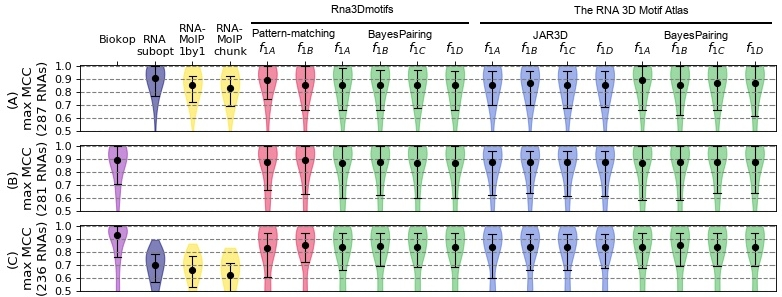
\includegraphics[width=\textwidth]{Benchmark_unconstrained.jpg}
   \caption{\textcolor{red}{First, second and third quartiles of the max MCC for each RNA, for all tools and BiORSEO variants.} 
   (A); Results of the methods that cannot find pseudoknots on the RNA-Strand dataset: RNAsubopt, RNA-MoIP, and the 14 variants of BiORSEO's bi-objective methods with a constraint that explicitly forbids pseudoknots. 
   (B); Results of the methods which allow pseudoknot predictions on the RNA-Strand dataset: Biokop, and the 14 BiORSEO variants without the no-pseudoknot constraint. 
   (C); Results of every method on the Pseudobase dataset. 
   \textcolor{red}{Due to the combinatorial issues commented in section \ref{sec:mat}, we counted only RNAs that could be predicted with every method: 287/344 in (A), 281/344 in (B), and 236/264 in (C).}}
   \label{fig:benchmark}
\end{figure*}
All the method \textcolor{red}{variants} introduced return an ensemble of possible secondary structures \textcolor{red}{(the Pareto set)} for a given input sequence. 
We compare them in a benchmark. \textcolor{red}{A small case study on three well known RNAs can be found in Supplementary Section D.}
\subsection{Benchmark protocol} \label{sec:bench}

\paragraph{Benchmark data sources} \label{sec:data}
A first dataset of RNA secondary structures was extracted from the RNA-Strand database ~(\citealp{andronescu2008rna}). We selected the RNAs for which experimental proof of the structure exists, with size varying between 10 and 100 nucleotides. Sequences containing modified nucleotides were discarded. The resulting set contains 344 secondary structures of various RNA families, 74 of them containing pseudoknots. We repeated the experiments twice: first, by forbidding explicitly the formation of pseudoknots with additional constraints (for fair comparison with RNA-MoIP). 
Then, a second experiment without such limitation, to reach maximum performance. In addition, to explicitly assess the performance on pseudoknotted RNAs, methods were tested on a second collection of 264 pseudoknotted-only RNAs from the Pseudobase database~(\citealp{van2000pseudobase}), covering all pseudoknot families, and of the same length range.

\paragraph{Reference comparison methods}
To study the usefulness of the module data sources, objective functions, and module placement methods, we added state-of-the art tools to the comparison. 
The same RNA sequences were submitted to RNAsubopt + RNA-MoIP for direct performance comparison. 
\textcolor{red}{In 'one by one' mode, RNA-MoIP inserts modules in every solution from RNAsubopt one by one, and we select the best solution ourselves like we do with BiORSEO (see the following paragraph \textit{Metrics}). In 'chunk' mode, RNA-MoIP takes all the RNAsubopt predictions at once and returns only one solution, supposed to be the best in the input set according to its own objective function.} 
We used RNAsubopt as a reference method without pseudoknot support, because it is fast, widely used, easy to understand and returns several solutions \textcolor{red}{that are in an energy range from the MFE (default parameter used)}. 
We used Biokop, \textcolor{red}{another} bi-objective ILP framework, as a reference method for prediction of secondary structures with pseudoknots. 
Both tools \textcolor{red}{RNAsubopt and Biokop out-perform} other state-of-the-art tools in their respective categories \textcolor{red}{(see  (\citealp{lorenz2011viennarna}) and  (\citealp{legendre_bi-objective_2018})} for more benchmarks against other tools\textcolor{red}{)}.

\paragraph{Metrics} ~ We compute the Matthews correlation coefficient (MCC) between the real secondary structure and every proposed structure. 
The coefficient is defined as:
{\small
\begin{equation}
   MCC = \frac{TP. TN - FP. FN}{\sqrt{(TP+FP)(TP+FN)(TN+FP)(TN+FN)}}. \label{eq:MCC}
\end{equation}
}\noindent
where TP, TN, FP and FN are the number of true/false positive and negative predicted base pairs.
\textcolor{red}{The choice of MCC over accuracy or F1 score is justified by the large difference between the size of the classes: in any secondary structure, there exist much more pairs of nucleotides that do not interact than pairs that do.
Here, we wonder if the "true" structure (which is only a possible state that has been observed and reported in a database) can be found in the Pareto set.
Therefore, we chose to keep the maximum MCC value found over the set of proposed structures as a metric of the method's performance, showing that a solution is close or not to this "true" structure. This is, to our knowledge, the best way to relate if the reference structure is part of our ensemble of solutions.} For comprehensiveness, results with average MCC are also provided in Supplementary Section E. 


\subsection{Benchmark results}
Performance results under the form of \textcolor{red}{maximum} MCC are summarized in Figure \ref{fig:benchmark}. No data source, nor objective function taken alone performs significantly better than the other ones.
Without pseudoknots, RNAsubopt out-performs the other tools (see Figure \ref{fig:benchmark}(A)). The second most performing model is \textcolor{red}{BiORSEO, using Rna3Dmotifs modules, placed by regular expression searches only, and scored with module size ($f_{1A}$). } With pseudoknots support, most of the RNAs are predicted with small pseudoknots as the method allows it. As Figure \ref{fig:benchmark}(B) shows, the methods \textcolor{red}{are still all very close in terms of performance, including Biokop} which performs \textcolor{red}{as well} without module information. \textcolor{red}{The best BiORSEO variant is the same, and it out-performs Biokop for 60 RNAs, which is only 17\% of the cases. }
The results on the dataset of pseudoknotted-only structures are presented on Figure~\ref{fig:benchmark}(C).
\textcolor{red}{Again}, the 14 variants are very close and no module source, pattern-matching method nor objective function distinguishes itself. \textcolor{red}{But this time, Biokop performs better in average.}

\paragraph{\textcolor{red}{Number of solutions}} ~ \textcolor{red}{As shown in Figure~\ref{fig:nsol}}, \textcolor{red}{all the BiORSEO models} return very small sets of unique secondary structures, some of them being one optimal solution sometimes for example when using JAR3D. Meanwhile, RNAsubopt returns from one to \textcolor{red}{tens} of solutions (with \textcolor{red}{default energy gap} settings)\textcolor{red}{, and Biokop even more. The RNA-MoIP goal is conserved here with our approach: identify a secondary structure among the MEA suboptimals (or a few, but rarely more than 5) based on its compatibility with known modules. Note that the selection of the max MCC solution in the results set naturally favors RNAsubopt and Biokop in our benchmark since they return way more solutions.}
\begin{figure}[!tbp]
  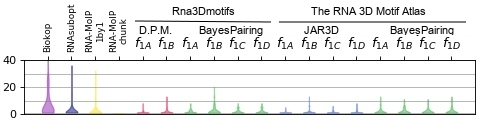
\includegraphics[width=\linewidth]{Nsol.jpg}
  \caption{\textcolor{red}{Number of unique secondary structures in the Pareto set or returned ensemble. Data is from the RNAStrand dataset. Pseudoknots are allowed. Note that this is not the size of the Pareto set, one unique secondary structure can often be found several times in the Pareto set, with different module combinations inserted in. The default RNA-MoIP usage, labelled "chunk" here, always returns only one solution selected by itself.}}
  \label{fig:nsol}
\end{figure}
\begin{figure}[!tbp]
  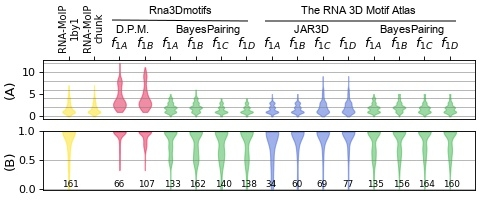
\includegraphics[width=\linewidth]{Nmotifs.jpg}
  \caption{\textcolor{red}{(A) Maximum number of modules inserted in a solution of the set. (B) Ratio of the number of modules inserted in the solution which is closest to the true structure (i.e. the max MCC solution) and the maximum number of inserted modules in a solution. Only RNAs for which the Pareto set contains more than one solution are counted (the count is given under the distribution). Data is from the RNAStrand dataset. Pseudoknots are allowed.}}
  \label{fig:info}
\end{figure}
\begin{figure*}[!tbp]
  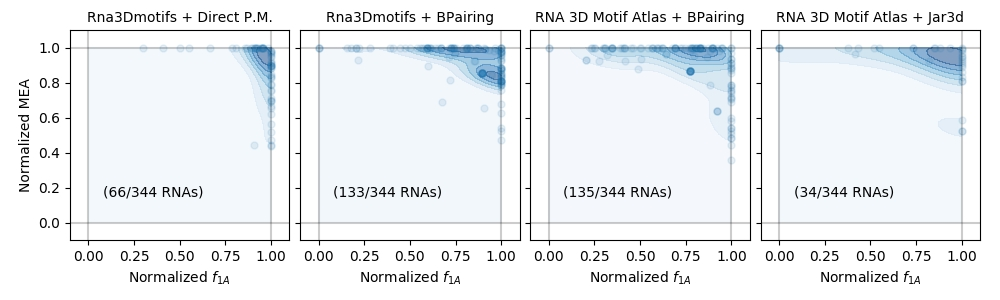
\includegraphics[width=\linewidth]{kernels_A.jpg}
  \caption{\textcolor{red}{Position of the best solution in the Pareto set for 4 variants using objective $f_{1A}$, after normalization on both axis. Computed on the RNA-Strand dataset with pseudoknots allowed. RNAs for which the Pareto set is a single optimal solution, or a set of solutions with the same secondary structure but different modules inserted into it, are ignored. The final number of considered RNAs is given on the figure.}}
  \label{fig:pareto}
\end{figure*}
\textcolor{red}{
\subsection{Usefulness of the two objectives}
To further study the RNA modules criteria usefulness, we looked at the maximum number of inserted modules over the Pareto solutions proposed for each RNA (Figure~\ref{fig:info}(A)), and the ratio between the number of inserted modules in the best prediction in the Pareto set (the max MCC solution) and this maximum number (Figure~\ref{fig:info}(B)).
When this ratio is 1, the best solution is the one with the most modules detected in (or one of the solutions with the most modules). The results show that in large majority, this ratio is 1. 
In particular, the variants which use direct pattern matching can insert more modules in average (up to 12) and this ratio is always at one. This is encouraging, showing that the best solutions do contain a lot of modules inserted.\\
Then, we display a solution space plot where we report the position of the best solution in the Pareto set after a normalization step, to directly observe where the best solutions are located in the MEA and RNA modules bi-objective plane. Variants which use $f_{1A}$ are presented on Figure \ref{fig:pareto}, plots for the other criteria are available in Supplementary Section F, they are close to what happens with $f_{1A}$. We only consider Pareto sets for which there exist more than one secondary structure solution in. 
First, we observe that the more Pareto sets we eliminate for this reason, the more the criteria are correlated, resulting in a single optimal solution. For example, we can say that $f_{1A}$ when used with JAR3D is correlated to MEA because in 312 cases on 344 an optimal secondary structure is found (most right plot on Figure~\ref{fig:pareto}). The eight variants which use BayesPairing are the less correlated with MEA, resulting in well spread positions of the best solution across the solution space. 
But the most interesting variant is Rna3Dmotifs + direct pattern-matching + $f_{1A}$, which performs the best. When several secondary structures are proposed, the best one is more often on the module criteria side than the MEA (most left plot on Figure~\ref{fig:pareto}; most of the best solutions have an abscissa of 1.0 or close). Therefore in this variant's case, when the criteria are not perfectly correlated, $f_{1A}$ is able to select the good solutions which are not the best on MEA.
}

%%%%%%%%%%%%%%%%%%%%%%%%%%%%%%%%%%%%%%%%%%%%%%%%%%%%%%%%%%%%%%%%%%%%%%%%%%%%%%%%%%%%%%%%%%%%%%%%%%%%
%%%%%%%%%%%%%%%%%%%%%%%%%%%%%%%%%%%%%%%%%%%%%%%%%%%%%%%%%%%%%%%%%%%%%%%%%%%%%%%%%%%%%%%%%%%%%%%%%%%%
\section{Discussion}
\paragraph{Comparison to RNA-MoIP} ~  An interesting point is the improvement between RNA-MoIP and our bi-objective variant which uses direct-pattern matching to spot insertion sites and $f_{1A}$ to score the insertions. This variant only differs from RNA-MoIP because it is bi-objective.  
Then, the Pareto approach really improves the structure prediction by itself. This result supports our hypothesis about RNA-MoIP breaking important basepairs.

\paragraph{\textcolor{red}{About pseudoknots predictions}} ~ 
The support of pseudoknots \textcolor{red}{and a lower number of solutions returned are the real interesting features} about BiORSEO. \textcolor{red}{It returns several} solutions, some with pseudoknots, and some without. As we are looking at the max MCC here, the appropriate solution is selected for each RNA. \textcolor{red}{Fortunately, the number of solutions returned is always smaller than the state-of-the-art tools. This makes the use of the maximum MCC acceptable as a metric.}
However, pseudoknot prediction quality is still difficult to assess with a metric like MCC, because a pseudoknot could be involving only a few base-pairs. Finding them or not does not alter much the MCC even if the structure is much more right or wrong from a biological point of view. Unfortunately, no automated verification method exists yet to our knowledge. \textcolor{red}{We illustrate this issue with the G riboswitch pseudoknot example in Supplementary Sections D2 and D3. The pseudoknot is sometimes found, but not with the exact same list of basepairs, which is penalized by the MCC.} 
\paragraph{\textcolor{red}{About RNA modules}}
\textcolor{red}{
On one side, the state-of-the-art~(\citealp{reinharz_towards_2012, theis2015rna}), the number of inserted modules in the best solutions (Figure \ref{fig:info}), and the position of the best solutions in the Pareto sets (Figure \ref{fig:pareto}) argue that criteria related to known modules are relevant. They should bring information from data to assist the theoretical model. But on the other side, Biokop is  \textit{in fine} equal or above BiORSEO in terms of performance, while Biokop does not use modules. The simplest explanation is that the MFE criterion it uses is important, and we lost information when we replaced it by a module criterion in BiORSEO.
}

\paragraph{On the objective functions} ~ 
Regarding objective functions to include modules, the different criteria proposed seem to give comparable results at first sight regarding the average performance and the dispersion. However, an important difference between $f_{1A}$, $f_{1B}$ on one side, and $f_{1C}$, $f_{1D}$ on the other side, is about the computation time. As $f_{1A}$, $f_{1B}$ do not use a score to rank potential module insertion sites, every module of the same size can be equally inserted. When the RNA presents several loops, the combinatorial possibilities grow fast with the number of modules in the dataset. Therefore, the number of undominated solutions can reach several hundreds or thousands even for short sequences. Such large Pareto sets are not informative for our application, because they consist \textcolor{red}{of} very redundant secondary structures with different module references, which are counted only for one secondary structure solution at the end. On the other hand, $f_{1C}$ and $f_{1D}$ require the run of an additional tool (JAR3D or BayesPairing) to score the insertion sites. Given an RNA, a compromise must be found according to its length and amount of loops.

\paragraph{The bias with JAR3D} ~ One should keep in mind that JAR3D takes as input the sequences of RNA loops to score modules against them. We detect the loops in the RNA sequence with RNAsubopt. This use of JAR3D is biased, since we score modules on sequence portions that we already know likely to form loops and  unlikely to form stems, so the information brought by a module insertion is low. \textcolor{red}{This is why we find it correlated to MEA.}

\paragraph{About BayesPairing} ~ Please remind that we skipped BayesPairing's last step which checks if the insertion of a module would deteriorate too much the energy. We did so because our bi-objective framework was supposed to be able to do it itself. The low performance of BayesPairing in the benchmark is not an argument against it when used in its intended purpose.

\paragraph{Computation times and material limits} \label{sec:mat}~ 
As evocated in Figure \ref{fig:benchmark}, the methods were not all able to fold all the sequences. The missing ones often are from a combination of direct pattern-matching or JAR3D with $f_{1A}$ or $f_{1B}$. \textcolor{red}{On the other hand, direct-pattern matching with $f_{1B}$ and in particular $f_{1A}$ also are the fastest methods. Computation time examples are provided in the case study in Supplementary Section D.}
The RAM, not the time, typically limits the size of the RNAs the methods can process. RNAs up to 230 bases are fine \textcolor{red}{on our workstation with 16GB of RAM}. A prediction typically takes a few seconds, sometimes minutes. The time required grows with both the nucleotide count, the number of similar loops, and the number of similar modules insertible on those similar loops. The objective functions $f_{1A}$ and $f_{1B}$, which are not sequence-dependant, were sometimes not discriminative enough and equally ranked a large number of combinatorial ordering variations of the same modules on the same loops. For that reason, we had to arbitrarily stop the jobs exceeding 500 structures in the Pareto set, because they would require several hours to complete, leading to incomplete dataset predictions.

%%%%%%%%%%%%%%%%%%%%%%%%%%%%%%%%%%%%%%%%%%%%%%%%%%%%%%%%%%%%%%%%%%%%%%%%%%%%%%%%%%%%%%%%%%%%%%%%%%%%
%%%%%%%%%%%%%%%%%%%%%%%%%%%%%%%%%%%%%%%%%%%%%%%%%%%%%%%%%%%%%%%%%%%%%%%%%%%%%%%%%%%%%%%%%%%%%%%%%%%%
\vspace{-0.5cm}
\section{Conclusion}
We developed a general bi-objective method to benchmark different sources of RNA modules models (the RNA 3D Motif Atlas and Rna3Dmotif), different methods to place them in sequences (direct pattern matching, BayesPairing, and JAR3D), and different scoring functions. The bi-objective method uses \textcolor{red}{a theoretical criterion,} the expected accuracy of the structure, and \textcolor{red}{a data-based criterion, one of} the previous scoring functions, to select relevant secondary structures.

Our models \textcolor{red}{out-perform} RNA-MoIP, a previous attempt to predict better secondary structures using module information and a linear combination of two objectives into a scoring function. Our simplest best-performing new method \textcolor{red}{uses Rna3Dmotifs placed in sequences by regular expression searches and scored by module size. It} could be interpreted as an upgraded RNA-MoIP with a real bi-objective framework, which predicts the base pairs and the module insertions in a row, preventing the insertion to break important base-pairs. \textcolor{red}{However, no module model distinguishes itself from the other. Regarding module detection methods, JAR3D seems biased and results in correlated criteria. The use of direct pattern matching is simple and efficient but leads to combinatorial issues on some RNAs, because we cannot score the insertion sites so that one beats the other candidates. Even if no variant of the method has a better predictive performance than Biokop in average (which performs the same or better using MFE but no module information), the module criterion improves the prediction in  17\% of the cases.} \textcolor{red}{In a future work, we should then develop a tri-objective optimization program including MFE as another criterion.}

Improvement perspectives relies on the hope newer databases like CaRNAval~(\citealp{reinharz2018mining}) that contain more recent and more diverse module models \textcolor{red}{including real pseudoknotted interaction networks},
bring more information to assist the energy criteria. 

\begin{thebibliography}{25}
   \bibitem[Andronescu {\em et~al.}(2008)Andronescu, Bereg, Hoos, and
     Condon]{andronescu2008rna}
   Andronescu, M., Bereg, V., Hoos, H.~H., and Condon, A. (2008).
   \newblock Rna strand: the {RNA} secondary structure and statistical analysis
     database.
   \newblock {\em BMC bioinformatics\/}, {\bf 9}(1), 340.
   
   \bibitem[Bellaousov and Mathews(2010)Bellaousov and
     Mathews]{bellaousov2010probknot}
   Bellaousov, S. and Mathews, D.~H. (2010).
   \newblock Probknot: fast prediction of {RNA} secondary structure including
     pseudoknots.
   \newblock {\em RNA\/}, {\bf 16}(10), 1870--1880.
   
   \bibitem[Chojnowski {\em et~al.}(2014)Chojnowski, Wale{\'n}, and
     Bujnicki]{chojnowski2014rna}
   Chojnowski, G., Wale{\'n}, T., and Bujnicki, J.~M. (2014).
   \newblock Rna bricks-a database of {RNA} 3d motifs and their interactions.
   \newblock {\em Nucleic acids research\/}, {\bf 42}(D1), D123--D131.
   
   \bibitem[Cruz and Westhof(2011)Cruz and Westhof]{cruz2011sequence}
   Cruz, J.~A. and Westhof, E. (2011).
   \newblock Sequence-based identification of 3d structural modules in {RNA} with
     rmdetect.
   \newblock {\em Nature methods\/}, {\bf 8}(6), 513.
   
   \bibitem[Dirks and Pierce(2004)Dirks and
     Pierce]{dirksAlgorithmComputingNucleic2004}
   Dirks, R.~M. and Pierce, N.~A. (2004).
   \newblock An algorithm for computing nucleic acid base-pairing probabilities
     including pseudoknots.
   \newblock {\em Journal of Computational Chemistry\/}, {\bf 25}(10), 1295--1304.
   
   \bibitem[Djelloul and Denise(2008)Djelloul and Denise]{djelloul_automated_2008}
   Djelloul, M. and Denise, A. (2008).
   \newblock Automated motif extraction and classification in {RNA} tertiary
     structures.
   \newblock {\em RNA\/}, {\bf 14}(12), 2489--2497.

   \bibitem[Ge {\em et~al.}(2018)Ge, Islam, Zhong and Zhang]{ge2018novo}
   Ge, P., Islam, S., Zhong, C., and Zhang, S. (2018). 
   \newblock De novo discovery of structural motifs in RNA 3D structures through clustering. 
   \newblock {\em Nucleic acids research\/}, {\bf 46}(9), 4783--4793.
   
   \bibitem[Gendron {\em et~al.}(2001)Gendron, Lemieux, and
     Major]{gendron2001quantitative}
   Gendron, P., Lemieux, S., and Major, F. (2001).
   \newblock Quantitative analysis of nucleic acid three-dimensional structures.
   \newblock {\em Journal of molecular biology\/}, {\bf 308}(5), 919--936.
      
   \bibitem[Legendre {\em et~al.}(2018)Legendre, Angel, and
     Tahi]{legendre_bi-objective_2018}
   Legendre, A., Angel, E., and Tahi, F. (2018).
   \newblock Bi-objective integer programming for {RNA} secondary structure
     prediction with pseudoknots.
   \newblock {\em BMC Bioinformatics\/}, {\bf 19}(1), 13.
   
   \bibitem[Leontis and Westhof(2001)Leontis and Westhof]{leontis2001geometric}
   Leontis, N.~B. and Westhof, E. (2001).
   \newblock Geometric nomenclature and classification of {RNA} base pairs.
   \newblock {\em RNA\/}, {\bf 7}(4), 499--512.
      
   \bibitem[Lorenz {\em et~al.}(2011b)Lorenz, Bernhart, Zu~Siederdissen, Tafer,
     Flamm, Stadler, and Hofacker]{lorenz2011viennarna}
   Lorenz, R., Bernhart, S.~H., Zu~Siederdissen, C.~H., Tafer, H., Flamm, C.,
     Stadler, P.~F., and Hofacker, I.~L. (2011b).
   \newblock ViennaRNA Package 2.0.
   \newblock {\em Algorithms for Molecular Biology\/}, {\bf 6}(1), 26.
   
   \bibitem[Lu {\em et~al.}(2015)Lu, Bussemaker, and Olson]{lu_dssr:_2015}
   Lu, X.-J., Bussemaker, H.~J., and Olson, W.~K. (2015).
   \newblock {DSSR}: an integrated software tool for dissecting the spatial
     structure of {RNA}.
   \newblock {\em Nucleic Acids Research\/}, {\bf 43}(21), e142--e142.
   
   \bibitem[Mathews(2004)Mathews]{mathews2004using}
   Mathews, D.~H. (2004).
   \newblock Using an {RNA} secondary structure partition function to determine
     confidence in base pairs predicted by free energy minimization.
   \newblock {\em RNA\/}, {\bf 10}(8), 1178--1190.
   
   \bibitem[McCaskill(1990)McCaskill]{mccaskill1990equilibrium}
   McCaskill, J.~S. (1990).
   \newblock The equilibrium partition function and base pair binding
     probabilities for {RNA} secondary structure.
   \newblock {\em Biopolymers: Original Research on Biomolecules\/}, {\bf
     29}(6-7), 1105--1119.
   
   \bibitem[Parisien and Major(2008)Parisien and Major]{parisien2008mc}
   Parisien, M. and Major, F. (2008).
   \newblock The mc-fold and mc-sym pipeline infers {RNA} structure from sequence
     data.
   \newblock {\em Nature\/}, {\bf 452}(7183), 51.
   
   \bibitem[Petrov {\em et~al.}(2013)Petrov, Zirbel, and
     Leontis]{petrov_automated_2013}
   Petrov, A.~I., Zirbel, C.~L., and Leontis, N.~B. (2013).
   \newblock Automated classification of {RNA} 3d motifs and the {RNA} 3d {Motif}
     {Atlas}.
   \newblock {\em RNA\/}, {\bf 19}(10), 1327--1340.
   
   \bibitem[Reinharz {\em et~al.}(2012)Reinharz, Major, and
     Waldisp{\"u}hl]{reinharz_towards_2012}
   Reinharz, V., Major, F., and Waldisp{\"u}hl, J. (2012).
   \newblock Towards 3d structure prediction of large {RNA} molecules: an integer
     programming framework to insert local 3d motifs in {RNA} secondary structure.
   \newblock {\em Bioinformatics\/}, {\bf 28}(12), i207--i214.
   
   \bibitem[Reinharz {\em et~al.}(2018)Reinharz, Soul{\'e}, Westhof,
     Waldisp{\"u}hl, and Denise]{reinharz2018mining}
   Reinharz, V., Soul{\'e}, A., Westhof, E., Waldisp{\"u}hl, J., and Denise, A.
     (2018).
   \newblock Mining for recurrent long-range interactions in {RNA} structures
     reveals embedded hierarchies in network families.
   \newblock {\em Nucleic Acids Research\/}, {\bf 46}(8), 3841--3851.
   
   \bibitem[Sarrazin-Gendron {\em et~al.}(2019)Sarrazin-Gendron, Reinharz, Oliver,
     Moitessier, and Waldisp{\"u}hl]{sarrazin2019automated}
   Sarrazin-Gendron, R., Reinharz, V., Oliver, C.~G., Moitessier, N., and
     Waldisp{\"u}hl, J. (2019).
   \newblock Automated, customizable and efficient identification of 3d base pair
     modules with bayespairing.
   \newblock {\em Nucleic acids research\/}.
   
   \bibitem[Sarver {\em et~al.}(2008)Sarver, Zirbel, Stombaugh, Mokdad, and
     Leontis]{sarver_fr3d:_2008}
   Sarver, M., Zirbel, C.~L., Stombaugh, J., Mokdad, A., and Leontis, N.~B.
     (2008).
   \newblock {FR}3d: finding local and composite recurrent structural motifs in
     {RNA} 3d structures.
   \newblock {\em Journal of Mathematical Biology\/}, {\bf 56}(1), 215--252.
   
   \bibitem[Sato {\em et~al.}(2011)Sato, Kato, Hamada, Akutsu, and
     Asai]{sato_ipknot:_2011}
   Sato, K., Kato, Y., Hamada, M., Akutsu, T., and Asai, K. (2011).
   \newblock {IPknot}: fast and accurate prediction of {RNA} secondary structures
     with pseudoknots using integer programming.
   \newblock {\em Bioinformatics\/}, {\bf 27}(13), i85--i93.
   
   \bibitem[Schlick(2018)Schlick]{schlick2018adventures}
   Schlick, T. (2018).
   \newblock Adventures with {RNA} graphs.
   \newblock {\em Methods\/}, {\bf 143}, 16--33.
   
   \bibitem[Theis {\em et~al.}(2013)Theis, Zu Siederdissen, Hofacker and Gorodkin]{theis2013automated}
   Theis, C., Zu Siederdissen, C., Hofacker, I. L., and Gorodkin, J. (2013). 
   \newblock Automated identification of RNA 3D modules with discriminative power in RNA structural alignments. 
   \newblock {\em Nucleic acids research\/}, {\bf 41}(22), 9999--10009.

   \bibitem[Theis {\em et~al.}(2015)Theis, Zirbel, Zu Siederdisse, Anthon, Hofacker, Nielsen and Gorodkin]{theis2015rna}
   Theis, C., Zirbel, C. L., Zu Siederdissen, C. H., Anthon, C., Hofacker, I. L., Nielsen, H., and Gorodkin, J. (2015). 
   \newblock RNA 3D modules in genome-wide predictions of RNA 2D structure. 
   \newblock {\em PloS One}, {\bf 10}(10), e0139900.

   \bibitem[Van~Batenburg {\em et~al.}(2000)Van~Batenburg, Gultyaev, Pleij, Ng,
     and Oliehoek]{van2000pseudobase}
   Van~Batenburg, F., Gultyaev, A.~P., Pleij, C., Ng, J., and Oliehoek, J. (2000).
   \newblock Pseudobase: a database with rna pseudoknots.
   \newblock {\em Nucleic Acids Research\/}, {\bf 28}(1), 201--204.
   
   \bibitem[Zirbel {\em et~al.}(2015)Zirbel, Roll, Sweeney, Petrov, Pirrung, and
     Leontis]{zirbel_identifying_2015}
   Zirbel, C.~L., Roll, J., Sweeney, B.~A., Petrov, A.~I., Pirrung, M., and
     Leontis, N.~B. (2015).
   \newblock Identifying novel sequence variants of {RNA} 3d motifs.
   \newblock {\em Nucleic Acids Research\/}, {\bf 43}(15), 7504--7520.
   
   \end{thebibliography}
   

\end{document}
